\section{Linear Search methods}

\begin{frame}
  \begin{itemize}
    \item Linear search

      На каждой итерации решается оптимизационная задача вдоль направления:

      \begin{align*}
        & f : \mathbb{R}^n \rightarrow  \mathbb{R} \\
        & \alpha = \argmin f(x_k + \alpha p_k)  \\
        & p_k = - B_{k}^{-1} \nabla f(x_k) 
      \end{align*}
    $B_k$ -- симметричная и невырожденная.
  \end{itemize}
\end{frame}


\subsection{Conditions}

\begin{frame}
  \begin{itemize}

  \item Armijo condition

    \begin{equation} \label{armijo}
    f(x_k + \alpha p_k) \leq f(x_k) + c_1 \alpha \nabla f_{k}^\intercal p_k, \; c_1 \in (0,1)
  \end{equation}

  \item curvature condition

    \begin{equation} \label{curvature}
    \nabla f(x_k + \alpha p_k)^\intercal p_k \geq c_2 \nabla f_{k}^\intercal p_k, \; c_2 \in (c_1, 1)
  \end{equation}

\item Wolfe condition: (\ref{armijo}) + (\ref{curvature})
  \end{itemize}

\end{frame}


\begin{frame}

  \begin{equation*}
    f(x_k + \alpha p_k) \leq f(x_k) + c_1 \alpha \nabla f_{k}^\intercal p_k, \; c_1 \in (0,1)
  \end{equation*}

\begin{figure}
\begin{minipage}{0.48\textwidth}
\centering
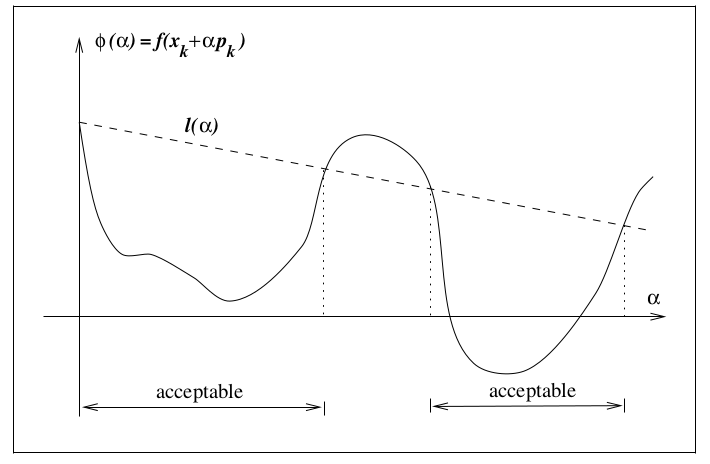
\includegraphics[height=3cm]{figures/armijo.png}
\end{minipage}
\begin{minipage}{0.48\textwidth}
\centering
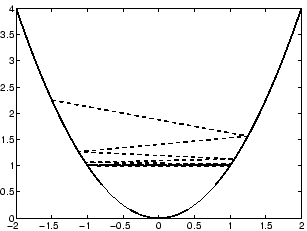
\includegraphics[height=3cm]{figures/armijo2.png}
\end{minipage}

\end{figure}

  \begin{equation*}
    l(\alpha) = f(x_k) + c_1 \alpha \nabla f_{k}^\intercal p_k, \; c_1 \in (0,1)
  \end{equation*}


\end{frame}

\begin{frame}
  \begin{equation*}
    \nabla f(x_k + \alpha p_k)^\intercal p_k \geq c_2 \nabla f_{k}^\intercal p_k, \; c_2 \in (c_1, 1)
  \end{equation*}

\begin{figure}
  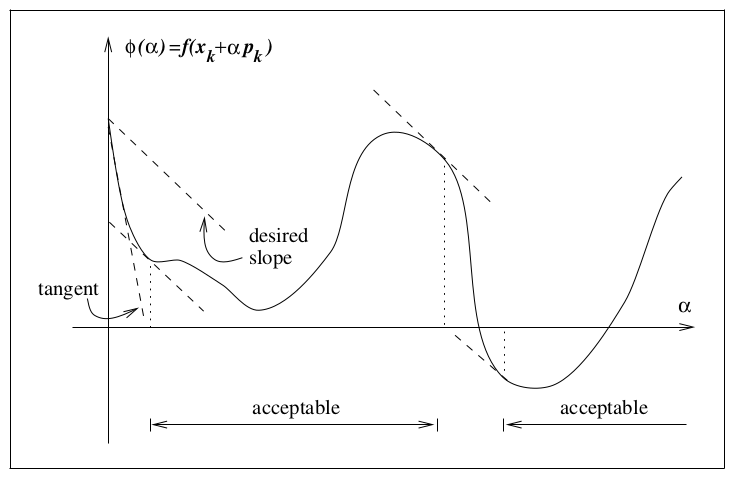
\includegraphics[height=5cm]{figures/curva.png}
\end{figure}

\end{frame}

\begin{frame}
  \frametitle{Strong Wolfe}
    \begin{equation*}
    f(x_k + \alpha p_k) \leq f(x_k) + c_1 \alpha \nabla f_{k}^\intercal p_k, \; c_1 \in (0,1)
  \end{equation*}

  \begin{equation*}
    \left| \nabla f(x_k + \alpha p_k)^\intercal p_k \right| \leq c_2 \left| \nabla f_{k}^\intercal p_k, \right| \; c_2 \in (c_1, 1)
  \end{equation*}

\begin{figure}
  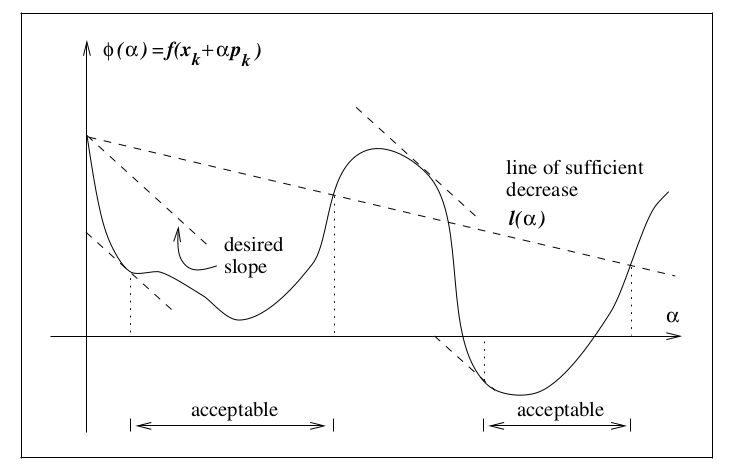
\includegraphics[height=5cm]{figures/strongWolfe.png}
\end{figure}

\end{frame}


\subsection{Step size selection}

\begin{frame}
  \frametitle{Intrepolation}
    \begin{equation*}
      \phi (\alpha_k) \leq \phi(0) + c_1 \alpha_k \phi'(0)
    \end{equation*}

    Как только $\alpha_k$ удовлетворяет условию, сразу прекращаем поиск.
    \begin{itemize}
    \item квадратичная аппроксимация

    \begin{equation*}
      \phi_q(\alpha) = \frac{\phi(\alpha_0) - \phi(0) - \alpha_0 \phi'(0)}{\alpha_0^2} \alpha^2 + \phi'(0) \alpha + \phi(0)
    \end{equation*}

    \item кубическая аппроксимация
      \begin{equation*}
        \phi_c(\alpha) = a \alpha^3 + b \alpha^2 + \phi'(0) \alpha + \phi(0)
      \end{equation*}
  \end{itemize}
\end{frame}



\subsection{Gradient descent}

\begin{frame}
  \frametitle{Градиентный спуск}
  \begin{itemize}

    \item  Задача:

    \begin{align*}
      F : \mathbb{R}^n \rightarrow \mathbb{R} \\
      x = \argmin F(x)
    \end{align*}
   
    \item Правило приближения:

    \begin{equation*}
      x_{k+1} = x_k - \alpha_{k} \nabla F(x_k)
    \end{equation*}

    \end{itemize}
\end{frame}



\subsection{Non-linear conjugate gradients}

%\subsubsection{Linear conjugate gradient method}
%
%\begin{frame}
%  \frametitle{Линейный метод сопряжённых градиентов}
%  \begin{equation*}
%    \min x^\intercal A x - x^\intercal b
%  \end{equation*}
%    $A$ -- симметричная и положительно определённая.
%  \begin{equation*}
%    \nabla f(x) = Ax - b
%  \end{equation*}
%
%  Вектора 
%
%\end{frame}
%
%\subsection{Non-linear conjugate gradients methdo}

\begin{frame}
   \frametitle{Нелинейный метод сопряжённых градиентов}
    \begin{align*}
      f : \mathbb{R}^n \rightarrow \mathbb{R} \\
      x = \argmin f(x)
    \end{align*}

    Решение:

    \begin{align*}
      & x _{k+1} = x_k + \alpha_k d_k \\
      & d_k = -\nabla f_k + \beta_k d_{k-1}
    \end{align*}

\end{frame}

\begin{frame}
  \frametitle{Выбор $\beta_k$}

  \begin{itemize}
    \item The Fletcher-Reeves method

      \begin{equation*}
        \beta_k^{FR} = \frac{\nabla f_k^\intercal \nabla f_k}{\nabla f_{k-1}^\intercal \nabla f_{k-1} }
      \end{equation*}
    \item The Polak-Ribiere method

      \begin{equation*}
        \beta_k^{PR} = \frac{\nabla f_k^\intercal \left( \nabla f_k - \nabla f_{k-1} \right)}{\left\|\nabla f_{k-1} \right\|^2}
      \end{equation*}


  \end{itemize}

\end{frame}



\subsection{BFGS}

\begin{frame}
  \frametitle{BFGS}
    \begin{align*}
      f : \mathbb{R}^n \rightarrow \mathbb{R} \\
      x = \argmin f(x)
    \end{align*}

    На каждой итерации следующее приближение:

    \begin{equation*}
      m_k(p) = f_k + \nabla f_k^\intercal p_k + \frac{1}{2} p_k^\intercal B_k p_k
    \end{equation*}

    $B_k \in R^{n \times  n}$ -- симметричная и положительно определённая.  

\end{frame}

\begin{frame}
    Направление поиска:

    \begin{equation*}
      p_k = - B_k^{-1} \nabla f_k
    \end{equation*}
    
    Новая точка:

    \begin{equation*}
      x_{k+1} = x_k + \alpha_k p_k
    \end{equation*}

    $\alpha_k$ -- выбирается с учетом Wolfe condition.

    $B_k$ -- не пересчитывается, а обновляется, учитывая кривизну функции с прошедшего шага.
\end{frame}

\begin{frame}
  \frametitle{Secant equation}
  
  После построения $m_{k+1}$ градиент $m_{k+1}$ должен совпадать с градиентом $f$ в $x_{k+1}$ и $x_k$.

  \begin{equation*}
    \nabla m_{k+1} (-\alpha_k p_k) = \nabla f_{k+1} - \alpha_k B_{k+1} p_k = \nabla f_k 
  \end{equation*}

  Откуда 

  \begin{equation*}
    B_{k+1} s_k = y_k
  \end{equation*}

  Мы хотим,чтобы  $B_k$ была положительно определенной 

  \begin{equation} \label{BFGS_secant}
    s_k^\intercal y_k > 0
  \end{equation}

  При выборе шага, удовлетворяющего Wolfe condition (\ref{BFGS_secant}) -- выполнятеся автоматически.
\end{frame}

\begin{frame}
  \frametitle{Выбор $B_{k+1}$}
      \begin{equation*}
        H_k = B_k^{-1} 
      \end{equation*}
      \begin{align*}
        &\min_H \left\| H - H_k \right\|_W \\
        &H = H^\intercal
      \end{align*}
      \begin{align*}
        &H_{k+1} = \left( I - \rho_k s_k y_k^\intercal \right) H_k \left( I - \rho_k y_k s_k^\intercal \right) + \rho_k s_k s_k^\intercal \\
        &\rho_k = \frac{1}{y_k^\intercal s_k}
      \end{align*}

\end{frame}

\begin{frame}
  \frametitle{Initial hessian approximation}

  Нет магической формулы, которая была бы хороша для каждой ситуации.

  \begin{equation*}
    B = \frac{\left\| \nabla f_0 \right\|}{\alpha}  
  \end{equation*}

  \begin{equation*}
    B = \frac{y_1^\intercal y_1}{y_1^\intercal s_1} I
  \end{equation*}

  \begin{equation*}
    B = I
  \end{equation*}
\end{frame}




\subsection{L-BFGS}

\begin{frame}
  \frametitle{L-BFGS}
  Проблема: размерность $H_k$ можеть быть очень большой, поэтому предлагается не хранить матрицу целиком, а содержать только лишь $m$ пар $(s_k, y_k)$.

  \begin{align*}
    & x_{k+1} = x_k - \alpha_k H_k \nabla f_k \\
    & H_{k+1} = V_k^\intercal H_k V_k + \rho_k s_k s_k^\intercal \\
    & V_k = I - \rho_k y_k s_k^\intercal, \quad \rho_k = \frac{1}{y_k^\intercal s_k} \\
    & s_k = x_{k+1} - x_k, \quad y_k = \nabla f_{k+1} - \nabla f_k
  \end{align*}
\end{frame}

\begin{frame}

  \begin{align*}
    H_k & = \left( V_{k-1}^\intercal ... V_{k-m}^\intercal \right)H_k^0 \left(V_{k-m} ... V_{k-1} \right) \\
        & + \rho_{k-m}  \left( V_{k-1}^\intercal ... V_{k-m-1}^\intercal \right) s_{k-m} s_{k-1}^\intercal \left(V_{k-m-1} ... V_{k-1} \right) \\
        & + ... \\
        & + \rho_{k-1} s_{k-1} s_{k-1}^\intercal
  \end{align*}

  $H_k^0$ -- начальное приближение, может быть выбрано так же, как и для BFGS.

  \begin{equation*}
    H_k^0 = \frac{s_{k-1}^\intercal y_{k-1}}{y_{k-1}^\intercal y_{k-1}}
  \end{equation*}
  
  %Смысл в том, что это пытается оценить размер "настоящего" Гессиана в направлении предыдущего шага.
\end{frame}



\section{Derivative-free optimization}

\subsection{Nelder-Mead}

\begin{frame}
  \frametitle{Nelder-Mead}

  Метод оптимизации функций без ограничений. 
  
  Поиск экстремальной точки происходит путем операций по изменению симплекса.

  Алгоритм:
  \begin{enumerate}
    \item Сортировка вершин по значению функции в них. Определение $f_h$, $f_s$, $f_l$.
    \begin{align*}
      f_h = \max_j f_j, \quad f_s = \max_{j \neq h} f_j, \quad f_l = \min_{j \neq h, j\neq s} f_j
    \end{align*}

    \item Вычисление центроида без $x_h$
    \begin{equation*}
      c = \frac{\sum_{i \neq h}^{n+1} x_i}{n}
    \end{equation*}
    \item Трансформация симплекса.
  \end{enumerate}


\end{frame}

\begin{frame}
  \frametitle{Трансформации}
  \begin{itemize}
    \item reflection 

      $x_r = c + \alpha(c - x_h)$, если $f_l \leq f_r \leq f_s$, то меняем $x_h$ на $x_r$.
      \begin{figure}
      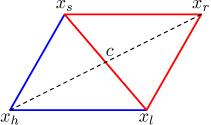
\includegraphics[height=2cm]{figures/reflection.jpg}
      \end{figure}

    \item expansion

    если $f_r < f_l$ то вычисляем $x_e = c + \gamma(x_r - c)$, если $f_e < f_r$, то меняем $x_h$ на $x_e$, иначе на $x_r$.
      \begin{figure}
      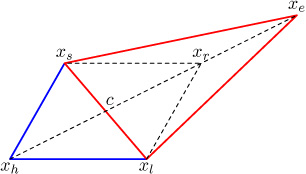
\includegraphics[height=2cm]{figures/expansion.jpg}
      \end{figure}

  \end{itemize}
\end{frame}

\begin{frame}
  \frametitle{Трансформации}
  \begin{itemize}
     \item Contraction

    при $f_r \geq f_l$ вычисляем $x_c$ используя меньшую из $f_r, f_h$ точку.

    $f_r < f_h$: $x_c = c + \beta(x_r - c)$, если  $f_c \leq f_r$ принимаем $x_c$ иначе shrink.

    $f_r \geq f_h$: $x_c = c + \beta(x_h - c)$, если  $f_c < f_h$ принимаем $x_c$ иначе shrink.

  \begin{figure}
    \begin{minipage}{0.4\textwidth}
      \centering
      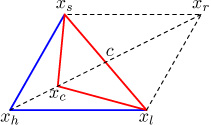
\includegraphics[height=2cm]{figures/contraction2.jpg}
    \end{minipage}
    \begin{minipage}{0.4\textwidth}
      \centering
      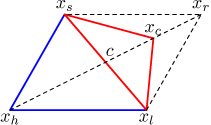
\includegraphics[height=2cm]{figures/contraction1.jpg}
    \end{minipage}
  \end{figure}
  \item Shrink

  Вычисляются n новых вершин симплекса : $x_j := x_l + \delta (x_j - x_l)$
       \begin{figure}
      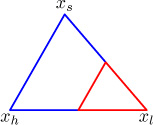
\includegraphics[height=2cm]{figures/shrink.jpg}
      \end{figure}
  
  \end{itemize}
\end{frame}


\begin{frame}
  \frametitle{Выбор начального симплекса}
  \begin{itemize}
    \item Выбирается начальное приближение экстремальной точки $x_0$.

    \begin{equation*}
      x_j = x_0 + h_j e_j,
    \end{equation*}

  $e_j$ -- направление, $h_j$ -- длина шага в направлении.


  \item Авторы оригинальной статьи предлагают строить правильный симплекс с одной из вершин в $x_0$.
\end{itemize}
\end{frame}


\section{KKT}

\subsection{Karush-Kuhn-Tucker conditions}

\begin{frame}
  \frametitle{Условия Каруша-Куна-Таккера}
  Задача:

  \begin{align*}
    & \min_x f(x) \\
    & l_j(x) \leq 0 \\
    & h_i(x) = 0
  \end{align*}
\end{frame}

\begin{frame}
  \begin{equation*}
    L(x,u,v) = f(x) + \sum_{i=1}^{m} u_i h_i(x) + \sum_{j=1}^{r} v_j l_j(x) 
  \end{equation*}

\begin{itemize}

\item Stationarity
\begin{align*}
  & \nabla L(x, u, v) = 0 
  \end{align*}

  \item Primal feasibility
\begin{align*}
  & l_j(x) \leq 0 \\
  & h_i(x) = 0 
\end{align*}

\item Dual feasibility
  \begin{align*}
    & u_i \geq 0 
  \end{align*}

\item Complementary slackness
\begin{align*}
  & u_i h_i(x) = 0
\end{align*}

\end{itemize}

\end{frame}

\begin{frame}

Если существует тройка $(x^*, u^*, v^*)$, удовлетворяющая условиям с прошлого слайда, то $x^*$ -- локальный минимум.

%\begin{figure}
%  \begin{minipage}{0.48\textwidth}
%  \centering
%  \includegraphics[height=3cm]{figures/kkt_slackness.png}
%  \caption{Complementary slackness}
%\end{minipage}
%\begin{minipage}{0.48\textwidth}
%  \centering
%  \includegraphics[height=3cm]{figures/dual_fis.png}
%  \caption{Dual feasibility}
%\end{minipage}
%
%\end{figure}


\end{frame}

